\documentclass[12pt, a4paper]{report}
% Verilog code formatting ref: https://tex.stackexchange.com/questions/377122/typesetting-for-a-verilog-lstinput
\usepackage{xcolor}
\usepackage{listings}
\definecolor{vgreen}{RGB}{104,180,104}
\definecolor{vblue}{RGB}{49,49,255}
\definecolor{vorange}{RGB}{255,143,102}

\lstdefinestyle{verilog-style}
{
    language=Verilog,    
    breaklines=true,    
    basicstyle=\small\ttfamily,
    keywordstyle=\color{vblue},
    identifierstyle=\color{black},
    commentstyle=\color{vgreen},
    numbers=left,
    numberstyle=\tiny\color{black},
    numbersep=10pt,
    tabsize=8,
    moredelim=*[s][\colorIndex]{[}{]},
    literate=*{:}{:}1
}

\definecolor{mGreen}{rgb}{0,0.6,0}
\definecolor{mGray}{rgb}{0.5,0.5,0.5}
\definecolor{mPurple}{rgb}{0.58,0,0.82}
\definecolor{backgroundColour}{rgb}{0.95,0.95,0.92}

\lstdefinestyle{CStyle}{
    backgroundcolor=\color{backgroundColour},   
    commentstyle=\color{mGreen},
    keywordstyle=\color{magenta},
    numberstyle=\tiny\color{mGray},
    stringstyle=\color{mPurple},
    basicstyle=\footnotesize,
    breakatwhitespace=false,         
    breaklines=true,                 
    captionpos=b,                    
    keepspaces=true,                 
    numbers=left,                    
    numbersep=5pt,                  
    showspaces=false,                
    showstringspaces=false,
    showtabs=false,                  
    tabsize=2,
    language=C
}

\makeatletter
\newcommand*\@lbracket{[}
\newcommand*\@rbracket{]}
\newcommand*\@colon{:}
\newcommand*\colorIndex{%
    \edef\@temp{\the\lst@token}%
    \ifx\@temp\@lbracket \color{black}%
    \else\ifx\@temp\@rbracket \color{black}%
    \else\ifx\@temp\@colon \color{black}%
    \else \color{vorange}%
    \fi\fi\fi
}
\makeatother
\usepackage{trace}

\setcounter{secnumdepth}{3} % To add subsubsections to the table of contents
% for QnA ref: https://latex.org/forum/viewtopic.php?t=10494
\newcounter{question}
\setcounter{question}{0}
\newcommand{\question}[1]{\item[\textbf{Q\refstepcounter{question}\thequestion.}] \textbf{#1}}
\newcommand{\answer}[1]{\item[Answer:] #1}


% A pretty common set of packages
\usepackage[margin=2.5cm]{geometry}
\usepackage[T1]{fontenc}
\usepackage[utf8]{inputenc}
\usepackage{blindtext}
\author{Maitreya Ranade}
\date{\today}
\usepackage{pdfpages}
\usepackage{graphicx}
\usepackage{amssymb}
\usepackage{amsmath}
\usepackage{color}
\usepackage{import}
\usepackage{booktabs}
\usepackage{multirow}
\usepackage{engord}
\usepackage{soul}
\usepackage{textcomp}
\usepackage{parskip}
\usepackage{setspace}
\usepackage{titlesec}
\usepackage{fancyhdr}
\usepackage{tabularx}
\usepackage{mathtools} % for '\DeclarePairedDelimiter' macro
\DeclarePairedDelimiter\norm\lVert\rVert
\usepackage{bookmark}
\pagestyle{fancy}
\usepackage[UKenglish]{babel}
\usepackage[UKenglish]{isodate}
\usepackage[skip=2pt,font=footnotesize,justification=centering]{caption}
\usepackage{natbib}
\usepackage{float}
\usepackage{dirtree}
\usepackage{url}
\usepackage{enumitem}
\usepackage{tgpagella}


% Custom environments
\newenvironment{highlight}
{\vspace{2mm} \hrule \vspace{2mm} \em}
{\vspace{2mm} \hrule \vspace{2mm}}


% Make some additional useful commands
\newcommand{\ie}{\emph{i.e.}\ }
\newcommand{\eg}{\emph{e.g.}\ }
\newcommand{\etal}{\emph{et al}}
\newcommand{\sub}[1]{$_{\textrm{#1}}$}
\newcommand{\super}[1]{$^{\textrm{#1}}$}
\newcommand{\degC}{$^{\circ}$C}
\newcommand{\wig}{$\sim$}
\newcommand{\ord}[1]{\engordnumber{#1}}
\newcommand{\num}[2]{$#1\,$#2}
\newcommand{\range}[3]{$#1$-$#2\,$#3}
\newcommand{\roughly}[2]{$\sim\!#1\,$#2}
\newcommand{\area}[3]{$#1 \! \times \! #2\,$#3}
\newcommand{\vol}[4]{$#1 \! \times \! #2 \! \times \! #3\,$#4}
\newcommand{\cube}[1]{$#1 \! \times \! #1 \! \times \! #1$}
\newcommand{\figref}[1]{Figure~\ref{#1}}
\newcommand{\eqnref}[1]{Equation~\ref{#1}}
\newcommand{\tableref}[1]{Table~\ref{#1}}
\newcommand{\secref}[1]{Section \ref{#1}}
\newcommand{\XC}{\emph{exchange-correlation}}
\newcommand{\abinit}{\emph{ab initio}}
\newcommand{\Abinit}{\emph{Ab initio}}
\newcommand{\Lonetwo}{L1$_{2}$}
\newcommand{\Dznt}{D0$_{19}$}
\newcommand{\Dtf}{D8$_{5}$}
\newcommand{\Btwo}{B$_{2}$}
\newcommand{\fcc}{\emph{fcc}}
\newcommand{\hcp}{\emph{hcp}}
\newcommand{\bcc}{\emph{bcc}}
\newcommand{\Ang}{{\AA}}
\newcommand{\inverseAng}{{\AA}$^{-1}$}
\newcommand{\comment}[1]{\textcolor{red}{[COMMENT: #1]}}
\newcommand{\more}{\textcolor{red}{[MORE]}}
\newcommand{\red}[1]{\textcolor{red}{#1}}
\newcommand{\SubItem}[1]{
    {\setlength\itemindent{15pt} \item[] \textbf{#1}}
}
% Change this to modify look of header and footer
\lhead{}
\chead{}
\rhead{}
\lfoot{}
\cfoot{\thepage{}}
\rfoot{}
\renewcommand{\headrulewidth}{0pt}
\renewcommand{\footrulewidth}{0pt}
\usepackage{hyperref}
\hypersetup{
    colorlinks=true,
    linkcolor=blue,
    filecolor=magenta,      
    urlcolor=cyan,
}
\urlstyle{same}
\newcommand{\foo}{\hspace{-2.3pt}$\bullet$ \hspace{5pt}}   % For timeline
  

\begin{document}
	\onehalfspacing
	Date: \today{} \hfill{} Name: Maitreya Ranade   
	\begin{center}
		\topskip0pt
		\vspace*{\fill}
		{\LARGE Zynq Documentation} \\
		This report is written for personal understanding and not for publication or distribution.
		\vspace*{\fill}
	\end{center}
	
	\pagebreak
	\singlespacing
	\tableofcontents
	\pagebreak


    \chapter{Zynq ultrascale+ MPsoc Architecture Overview}

    \section{Introduction to UltraScale Architecture}
    The Xilinx UltraScale architecture is the first ASIC-class architecture to enable
    multi-hundred gigabit-per-second levels of system performance with smart processing,
    while efficiently routing and processing data on-chip. UltraScale architecture-based devices
    address a vast spectrum of high-bandwidth, high-utilization system requirements by using
    industry-leading technical innovations, including next-generation routing, ASIC-like
    clocking, 3D-on-3D ICs, multiprocessor SoC (MPSoC) technologies, and new power
    reduction features. The devices share many building blocks, providing scalability across
    process nodes and product families to leverage system-level investment across platforms.


    Virtex UltraScale+ devices provide the highest performance and integration capabilities
    in a FinFET node, including both the highest serial I/O and signal processing bandwidth, as
    well as the highest on-chip memory density. As the industry's most capable FPGA family,
    the Virtex UltraScale+ devices are ideal for applications including 1+Tb/s networking and
    data center and fully integrated radar/early-warning systems.
    

    Virtex UltraScale devices provide the greatest performance and integration at 20 nm,
    including serial I/O bandwidth and logic capacity. As the industry's only high-end FPGA at
    the 20 nm process node, this family is ideal for applications including 400G networking,
    large scale ASIC prototyping, and emulation.


    Kintex UltraScale+ devices provide the best price/performance/watt balance in a FinFET
    node, delivering the most cost-effective solution for high-end capabilities, including
    transceiver and memory interface line rates as well as 100G connectivity cores. Our newest
    mid-range family is ideal for both packet processing and DSP-intensive functions and is well
    suited for applications including wireless MIMO technology, Nx100G networking, and data
    center.


    Kintex UltraScale devices provide the best price/performance/watt at 20 nm and include
    the highest signal processing bandwidth in a mid-range device, next-generation cost-effectiveness. 
    The family is ideal for packet processing in 100G networking and data
    centers applications as well as DSP-intensive processing needed in next-generation medical
    imaging, 8k4k video, and heterogeneous wireless infrastructure.


    Artix UltraScale+ devices provide high serial bandwidth and signal compute density in a
    cost-optimized device for critical networking applications, vision and video processing, and
    secured connectivity. Coupled with the innovative InFO packaging, which provides excellent
    thermal and power distribution, Artix UltraScale+ devices are perfectly suited to
    applications requiring high compute density in a small footprint.


    Zynq UltraScale+ devices provide 64-bit processor scalability while combining real-time
    control with soft and hard engines for graphics, video, waveform, and packet processing.
    Integrating an Arm-based system for advanced analytics and on-chip programmable
    logic for task acceleration creates unlimited possibilities for applications including 5G
    Wireless, next generation ADAS, and industrial Internet-of-Things.


    \chapter{Zynq ultrascale+ MPsoc Configurable logic blocks}


    \chapter{Zynq ultrascale+ MPsoc Clocking Resources}

    
    \section{Clocking Resource Abbreviations}
    \begin{itemize}
        \item CMT: clock management tile
        \item CR: clock region
        \item CLB: Configurable logic blocks
        \item HCS: Horizontal Clock Spine 
        \item GT: gigabit transceiver
        \item SYSMON: System Monitor
        \item MMCM: mixed-mode clock manager 
        \item PLL: phase-locked loop        
    \end{itemize}
    % \subsection{Clocking Overview}

    \section{Clocking Architecture Overview}
    The UltraScale architecture clocking resources manage complex and simple clocking requirements with dedicated global clocks distributed on clock routing and clock distribution resources. The clock management tiles (CMTs) provide clock frequency synthesis, deskew, and jitter filtering functionality. 

    \begin{itemize}
        \item The device is subdivided into columns and rows of segmented clock regions (CRs) which are arranged in tiles. A CR contains configurable logic blocks (CLBs), DSP slices, block RAMs, interconnect, and associated clocking. The height of a CR is 60 CLBs, 24 DSP slices, and 12 block RAMs with a Horizontal Clock Spine (HCS) at its center. The HCS contains the horizontal routing and distribution resources, leaf clock buffers, clock network interconnections, and the root of the clock network. Clock buffers drive directly into the HCS. There are 52 I/Os per bank and four gigabit transceivers (GTs)
        that are pitch matched to the CRs. A core column contains configuration, System
        Monitor (SYSMON), and PCIe blocks to complete a basic device.

        \item Adjacent to the input/output block columns are the physical layer (PHY) blocks with
        CMTs, global clock buffers, global clock multiplexing structures, and I/O logic management functions. The clocking drives vertical and horizontal connectivity
        through separate clock routing and clock distribution resources via HCS into the CRs
        and I/Os.
        \item Horizontal clock routing and distribution tracks drive horizontally into the CRs. Vertical
        routing and distribution tracks drive vertically adjacent CRs. The tracks are
        segmentable at the CR boundaries in both the horizontal and vertical directions. This
        allows for the creation of device-wide global clocks or local clocks of variable size.
        \item The distribution tracks drive the clocking of synchronous elements across the device.
        Distribution tracks are driven by routing tracks or directly by the clocking structures in
        the PHY.
        \item I/Os are directly driven from the PHY clocking and/or an adjacent PHY via routing
        tracks.
        \item A CMT contains one mixed-mode clock manager (MMCM) and two phase-locked loops
        (PLLs).
    \end{itemize}

    \section{Clocking Resources}
    \subsection{Overview}
    UltraScale architecture-based devices have several clock routing resources to support various clocking schemes and requirements, including high fanout, short propagation delay, and extremely low skew. To best utilize the clock routing resources, the designer must
    understand how to get user clocks from the PCB to the UltraScale devices, decide which clock routing resources are optimal, and then access those clock routing resources by utilizing the appropriate I/O and clock buffers.
    
    \subsection{Clock Routing Resources Overview}
    Each I/O bank contains global clock input pins to bring user clocks onto the device clock management and routing resources. The global clock inputs bring user clocks onto:
    \begin{itemize}
        \item Clock buffers in the PHY adjacent to the same bank
        \item CMTs in the PHY adjacent to the same bank
    \end{itemize}

    \subsection{Clock Buffers}
    Each device has three global clock buffers: BUFGCTRL, BUFGCE, and BUFGCE\_DIV. In addition, there is a local BUFCE\_LEAF clock buffer for driving leaf clocks from horizontal distribution to various blocks in the device. BUFGCTRL has derivative software representations of types BUFGMUX, BUFGMUX1, BUFGMUX\_CTRL, and BUFGCE\_1. BUFGCE is for glitchless clock gating and has software derivative BUFG (BUFGCE with clock enable tied High). The global clock buffers drive routing and distribution tracks into the device logic via HCS rows. There are 24 routing and 24 distribution tracks in each HCS row. There
    is also a BUFG\_GT that generates divided clocks for GT clocking. The clock buffers:

    \begin{itemize}
        \item Can be used as a clock enable circuit to enable or disable clocks either globally, locally, or within a CR for fine-grained power control.
        \item Can be used as a glitch-free multiplexer to:
        \begin{itemize}
            \item select between two clock sources.
            \item switch away from a failed clock source.
        \end{itemize}
        \item Are often driven by a CMT to:
        \begin{itemize}
            \item eliminate the clock distribution delay.
            \item adjust clock delay relative to another clock.
        \end{itemize}
    \end{itemize} 

    \subsection{Global Clock Inputs}
    External global user clocks must be brought into the UltraScale device on differential clock pin pairs called global clock (GC) inputs. There are four GC pin pairs in each bank that have direct access to the global clock buffers, MMCMs, and PLLs that are in the CMT adjacent to
    the same I/O bank. 
    
    GC inputs provide dedicated, high-speed access to the internal global and regional clock resources. GC inputs use dedicated routing
    and must be used for clock inputs where the timing of various clocking features is imperative. General-purpose I/O with local interconnects should not be used for clock signals.

    Each I/O bank is located in a single clock region and includes 52 I/O pins. Of the 52 I/O pins in each I/O bank in every I/O column, there are four global clock input pin pairs (a total of
    eight pins). Each global clock input:

    \begin{itemize}
        \item Can be connected to a differential or single-ended clock on the PCB.
        \item Can be configured for any I/O standard, including differential I/O standards.
        \item Has a P-side (master), and an N-side (slave).
    \end{itemize}

    Single-ended clock inputs must be assigned to the P (master) side of the GC input pin pair. If a single-ended clock is connected to the P-side of a differential clock pin pair, the N-side cannot be used as another single-ended clock pin—it can only be used as a user I/O. 
    
    GC inputs can be used as regular I/O if not used as clocks. When used as regular I/O, global clock input pins can be configured as any single-ended or differential I/O standard. GC inputs can connect to the PHY adjacent to the banks they reside in.

    \subsection{Byte Clock Inputs}
    Byte-lane clock (DBC and QBC) input pin pairs are dedicated clock inputs directly driving source synchronous clocks to the bit slices in the I/O banks. In memory applications, these are also known as DQS. When not used for I/O byte clocking these pin have other functions such as general purpose I/Os. 

    \subsection{Clock Buffers and Clock Routing}
    Global clocks are a dedicated network of interconnects specifically designed to reach all clock inputs to the various resources in a device. These networks are designed to have low skew and low duty cycle distortion, low power, and improved jitter tolerance. They are also designed to support very high-frequency signals.\\ 
    Understanding the signal path for a global clock expands the understanding of the various global clocking resources. The global clocking resources and network consist of these paths
    and components.
    \begin{itemize}
        \item Clock Structure
        \item Clock Buffers
        \item BUFGCTRL: Clock Buffer Primitives
        \item BUFGCE Clock Buffers
        \item BUFG Clock Buffer
        \item BUFCE\_LEAF Clock Buffer
    \end{itemize}

    \subsection{Clock Structure}
    The basic device architecture is composed of blocks of Clock Regions (CRs). CRs are organized into tiles and thus build columns and rows. Each CR contains slices (CLBs), DSPs, and 36K block RAM blocks.
    
    The mix of slice, DSP, and block RAM columns in each CR can be different, but are always identical when stacked in the vertical direction, thus building columns of those
    resources for the entire device. I/O and GT columns are then inserted with columns of CRs.
    In addition, there is a single column that contains the configuration logic, SYSMON, and PCIe blocks. An HCS runs horizontally through the device in the center of each row of CRs,
    I/Os, and GTs. The HCS contains the horizontal routing and distribution tracks as well as leaf
    clock buffers and clock network interconnects between horizontal/vertical routing and
    distribution. Vertical tracks of routing and distribution connect all CRs in a column, while
    vertical routing spans an entire I/O column. There are 24 horizontal routing and 24
    distribution tracks \figref{HorizClock}, and 24 vertical routing and 24 distribution tracks \figref{VertClock}. The purpose of the clock routing resources is to route a clock from the global
    clock buffers to a central point from where it is connected to the loads via the distribution
    resources. This central point of the clock network is called a clock root in the UltraScale
    architecture. The root can be in any CR in a device from where it is routed to the loads via
    the clock distribution resources. This architecture optimized clock skew. Routing and
    distribution resources can either connect to adjacent CRs or disconnect (isolated) at the
    border of the CR as needed. This concept extends to SSI devices as well.
    
    \begin{figure}[H]
        \begin{center}
            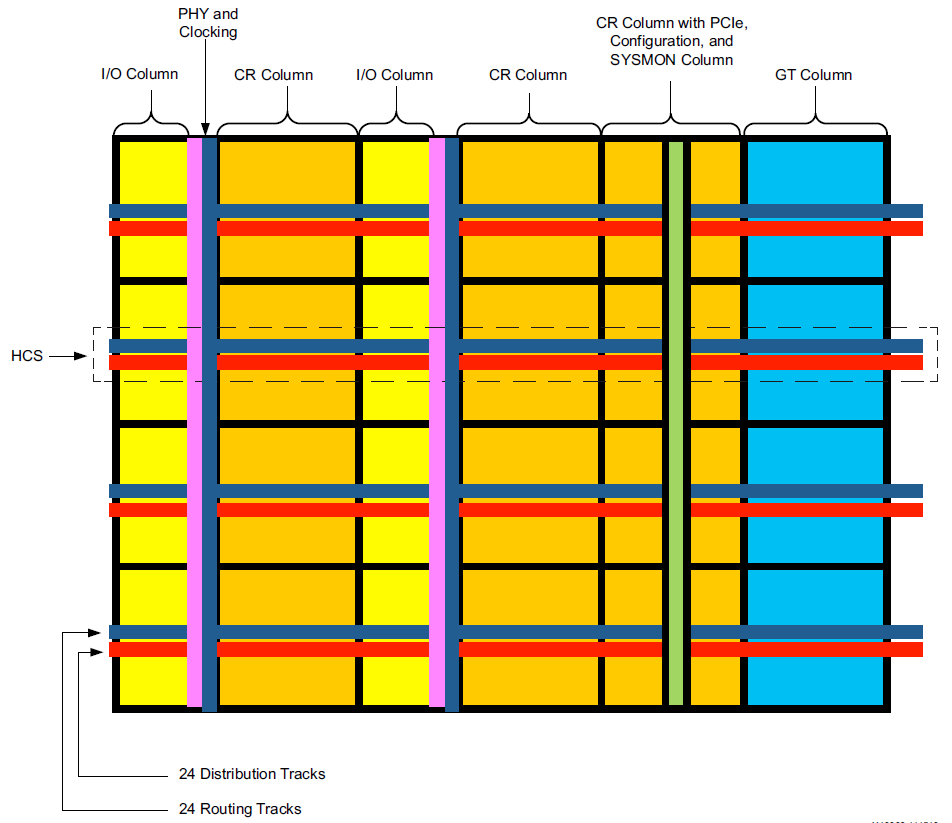
\includegraphics[width=0.7\textwidth]{images/HorizClock.png}
            \caption{Horizontal Clocking}
            \label{HorizClock}
        \end{center}
    \end{figure}

    \begin{figure}[H]
        \begin{center}
            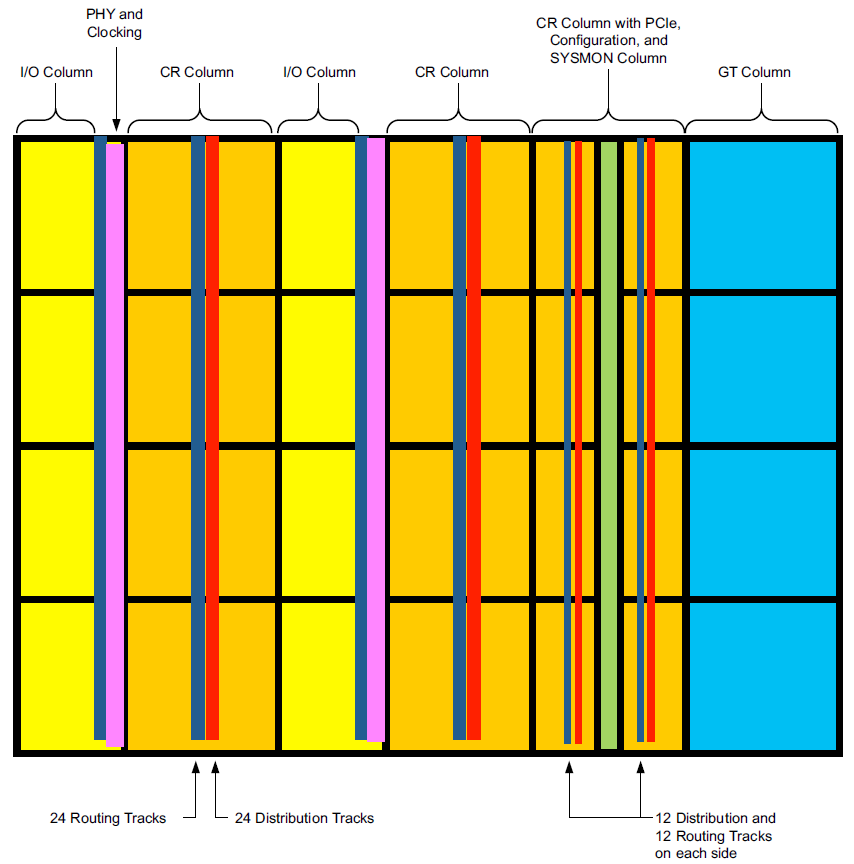
\includegraphics[width=0.7\textwidth]{images/VertClock.png}
            \caption{Vertical Clocking}
            \label{VertClock}
        \end{center}
    \end{figure}

    The clocks can be distributed from their sources in one of two ways:
    \begin{itemize}
        \item The clocks can go onto routing tracks that take the clocks to a central point in a CR
        without going to any loads. The clocks can then drive the distribution tracks
        unidirectionally from which the clock networks fan out. In this way, the clock buffers
        can drive to a specific point in the CRs from which the clock buffers travel vertically and
        then horizontally on the distribution tracks to drive the clocking points. The clocking points are driven via leaf clocks with clock enable (CE) in that CR and adjacent CRs, if
        needed. Distribution tracks cannot drive routing tracks.
        This distribution scheme is used to move the root for all the loads to be at a specific
        location for improved, localized skew. Furthermore, both routing and distribution tracks can drive into horizontally or vertically adjacent CRs in a segmented fashion. Routing
        tracks can drive both routing and distribution tracks in the adjacent CRs while the
        distribution tracks can drive other horizontal distribution tracks in adjacent CRs. The CR
        boundary segmentation allows construction of either truly global, device-wide clock
        networks or more local clock networks of variable sizes by reusing clocking tracks.

        \item Alternatively, clock buffers can drive straight onto the distribution tracks and distribute the clock in that manner. This reduces the clock insertion delay.
    \end{itemize}

    \begin{figure}[H]
        \begin{center}
            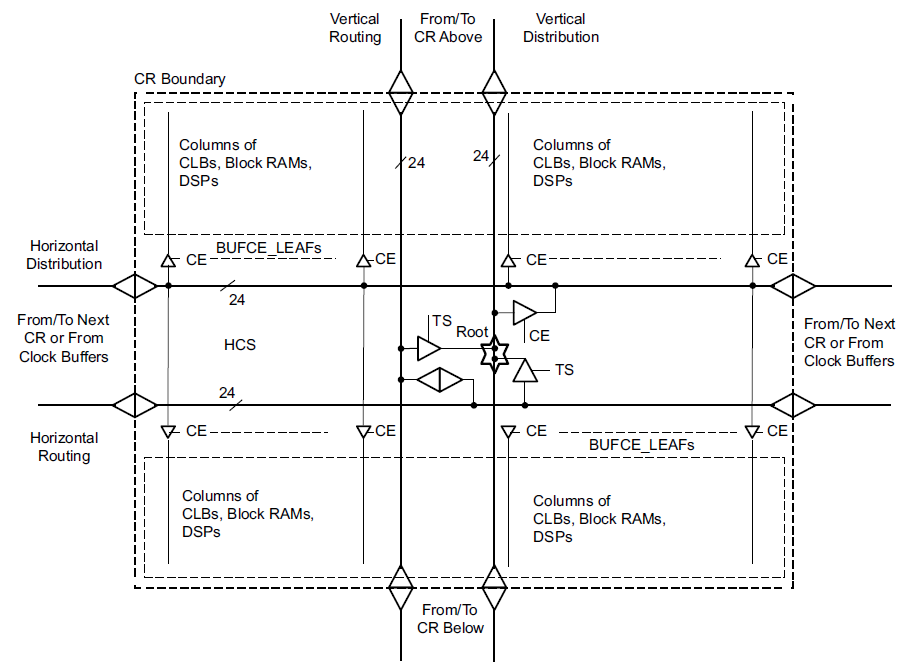
\includegraphics[width=0.7\textwidth]{images/clockDistr.png}
            \caption{Clock Distribution}
            \label{clockDistr}
        \end{center}
    \end{figure}


    \subsection{Clock Buffers}    
    The PHY global clocking contains several sets of BUFGCTRLs, BUFGCEs, and BUFGCE\_DIVs. Each set can be driven by four GC pins from the adjacent bank, MMCMs, PLLs in the same PHY, and interconnect. The clock buffers then drive the routing and distribution resources
    across the entire device. Each PHY contains 24 BUFGCEs, 8 BUFGCTRLs, and 4 BUFGCE\_DIVs  but only 24 of them can be used at the same time.

    \subsubsection{BUFGCTRL}
    The BUFGCTRL Clock Buffer Primitives are designed to switch between two clock inputs without the possibility of a glitch.     

    \begin{figure}[H]
        \begin{center}
            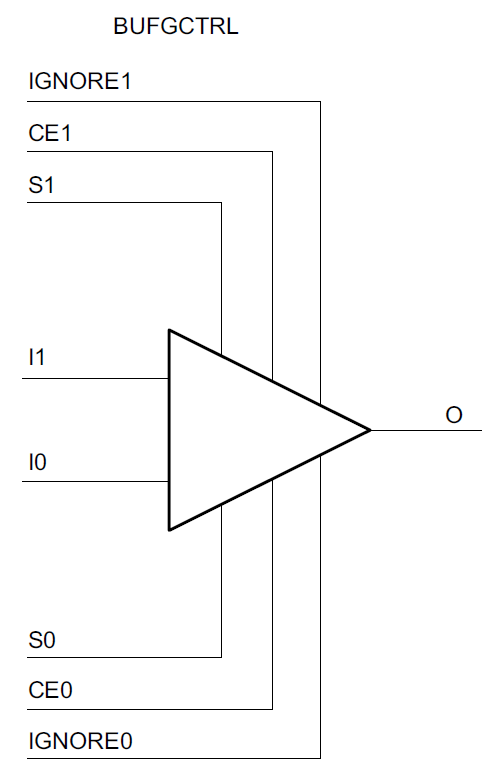
\includegraphics[width=0.7\textwidth]{images/BUFGCTRL.png}
            \caption{BUFGCTRL Clock Buffer Primitive}
            \label{BUFGCTRL}
        \end{center}
    \end{figure}
    
    All other global clock buffer primitives are derived from certain configurations of BUFGCTRL. Pins of the types of BUFGCTRL Clock Buffers:
    \begin{itemize}
        \item BUFGCTRL I0, I1 O CE0, CE1, IGNORE0, IGNORE1, S0, S1
        \item BUFGCE\_1 I O CE
        \item BUFGMUX I0, I1 O S
        \item BUFGMUX\_1 I0, I1 O S
        \item BUFGMUX\_CTRL I0, I1 O S
    \end{itemize}

    BUFGCTRL has four select lines, S0, S1, CE0, and CE1. It also has two additional control lines, IGNORE0 and IGNORE1. These six control lines are used to control the inputs I0 and I1.

    When the presently selected clock transitions from High to Low after S0 and S1 change, the output is kept Low until the other (to-be-selected) clock transitions from High to Low. Then, the new clock starts driving the output.

    \paragraph{BUFGCE\_1}
    BUFGCE\_1 is a clock buffer with one clock input, one clock output, and a clock enable line. This primitive is based on BUFGCTRL with some pins connected to logic High or Low.

    The switching condition for BUFGCE\_1 is similar to BUFGCTRL with INIT\_OUT set to 1. If the CE input is Low prior to the incoming falling clock edge, the following clock pulse does not
    pass through the clock buffer, and the output stays High. Any level change of CE during the incoming clock Low pulse has no effect until the clock transitions High. The output stays  High when the clock is disabled. However, when the clock is being disabled, it completes
    the clock Low pulse.
 
    \paragraph{BUFGMUX and BUFGMUX\_1}
    BUFGMUX is a clock buffer with two clock inputs, one clock output, and a select line (made by shorting CE0 \& CE1 lines). This primitive is based on BUFGCTRL with some pins connected to logic High or Low.

    \paragraph{BUFGMUX\_CTRL}
    BUFGMUX\_CTRL is a clock buffer with two clock inputs, one clock output, and a select line (made by shorting S0 \& S1 lines). This primitive is based on BUFGCTRL with some pins connected to logic High or Low. BUFGMUX\_CTRL uses the S pins as select pins. S can switch anytime without causing a
    glitch. The setup/hold time on S is for determining whether the output passes an extra pulse of the previously selected clock before switching to the new clock. If S changes prior to the setup time TBCCCK\_S and before I0 transitions from High
    to Low, the output does not pass an extra pulse of I0. If S changes following the hold time
    for S, the output passes an extra pulse. If S violates the setup/hold requirements, the output
    might pass the extra pulse but it will not glitch. In any case, the output changes to the new
    clock within three clock cycles of the slower clock.


    \subsubsection{BUFGCE}
    BUFGCE is a clock buffer with one clock input, one clock output, and a clock enable line. This buffer provides glitch-less clock gating. BUFGCE can directly drive the routing resources and is a clock buffer with a single gated input. Its output becomes 0 when CE goes Low (inactive). When CE goes High, the input is transferred to the output.

    BUFGCE Pins:
    \begin{itemize}
        \item CE: (Input) Clock enable
        \item I: (Input) Clock buffer
        \item O: (Output) Clock buffer
    \end{itemize}

    \subsubsection{BUFG}
    BUFG is a clock buffer with one clock input and one clock output. This primitive is based on BUFGCE with the CE pin connected to High.

    \subsubsection{BUFCE\_LEAF}
    BUFCE\_LEAF is a clock buffer with CE for leaf driving off horizontal HCS row. This buffer is an interconnect leaf clock buffer driving the clocking point of the various blocks with a single gated input. Its O output is 0 when CE is Low (inactive). When CE is High, the I input is
    transferred to the O output. 

    \subsubsection{BUFGCE\_DIV}
    BUFGCE\_DIV is a clock buffer with one clock input (I), one clock output (O), one clear input (CLR) and a clock enable (CE) input. BUFGCE\_DIV can directly drive the routing and distribution resources and is a clock buffer with a single gated input and a reset. 
    
    Its output is 0 when CLR is High (active). When CE is High, the input is transferred to the output. CE is synchronous to the clock for glitch-free operation. CLR is an asynchronous reset assertion and synchronous reset deassertion to this buffer.     
    
    BUFGCE\_DIV Pins:
    \begin{itemize}
        \item CE: (Input) Clock enable
        \item I: (Input) Clock buffer
        \item O: (Output) Clock buffer
        \item R: (Input) Reset
    \end{itemize}

    \subsubsection{BUFG\_GT and BUFG\_GT\_SYNC}
    The BUFG\_GTs are driven by the gigabit transceivers (GTs) and the ADC/DAC blocks in the RFSoC devices. BUFG\_GTs provide the only means for those blocks to drive the clock routing resources. Only GTs, ADCs, and DACs can drive BUFG\_GTs. BUFG\_GT is a clock
    buffer with one clock input (I), one clock output (O), one clear input (CLR) with CLR mask input (CLRMASK), a clock enable (CE) input with a CE mask input (CEMASK) and a 3-bit divide (DIV[2:0]) input. 
    
    BUFG\_GT\_SYNC is the synchronizer circuit for the BUFG\_GTs. The BUFG\_GT\_SYNC primitive is automatically inserted by the Vivado
    tools, if not present in the design. This buffer can directly drive the routing and distribution resources and is a clock buffer with a single gated input and a reset.     
    
    When CE is deasserted (Low) the output stops at its current state, High or Low. When CE is High, the I input is transferred to the O output. Both edges of CE and the deassertion of CLR are automatically
    synchronized to the clock for glitch-free operation. The Vivado tools do not support timing for the CE pin, therefore, a deterministic latency cannot be achieved. CLR is an asynchronous reset assertion and synchronous reset deassertion to the BUFG\_GTs. 

    \subsubsection{BUFG\_PS}
    The BUFG\_PS is a simple clock buffer with one clock input (I), one clock output (O). This clock buffer is a resource for the Zynq UltraScale+ MPSoC processor system (PS) and provides access to the programmable logic (PL) clock routing resources for clocks from the
    processor into the PL. Up to 18 PS clocks can drive the BUFG\_PS. This clock buffer resides next to the PS.


    \section{Clock Management Tile (CMT)}
    \subsection{Overview}
    In UltraScale architecture-based devices, each device has a CMT as part of the PHY next to each of the I/O banks. The clock management tile (CMT) includes a mixed-mode clock manager (MMCM) and two phase-locked loops (PLLs). 

    The MMCM is the primary block for frequency synthesis for a wide range of frequencies, and serves as a jitter filter for either external or internal clocks, and deskew clocks among a wide range of other functions.
    
    The main purpose of the PLL is to generate clocking for the I/Os. But it also contains a limited subset of the MMCM functions that can be used for general clocking purposes. The clock input connectivity allows multiple resources to provide the reference clock(s) to the MMCM. 
    
    MMCMs have infinite fine phase shift capability in either direction and can be used in dynamic phase shift mode. The resolution of the fine phase shift depends on the voltage-controlled oscillator (VCO)
    frequency.

    \subsection{MMCMs}
    The MMCMs serve as frequency synthesizers for a wide range of frequencies, and as jitter filters for either external or internal clocks, and deskew clocks. Input multiplexers select the reference and feedback clocks from either the global clock I/Os or the clock routing or distribution resources. Each clock input has a programmable counter divider (D). The phase-frequency detector (PFD) compares both phase and frequency of the rising edges of both the input (reference) clock and the feedback clock. If
    a minimum High/Low pulse is maintained, the duty cycle is ancillary. The PFD is used to
    generate a signal proportional to the phase and frequency between the two clocks. This
    the VCO. The PFD produces an up or down signal to the charge pump and loop filter to
    determine whether the VCO should operate at a higher or lower frequency.
    
    \begin{figure}[H]
        \begin{center}
            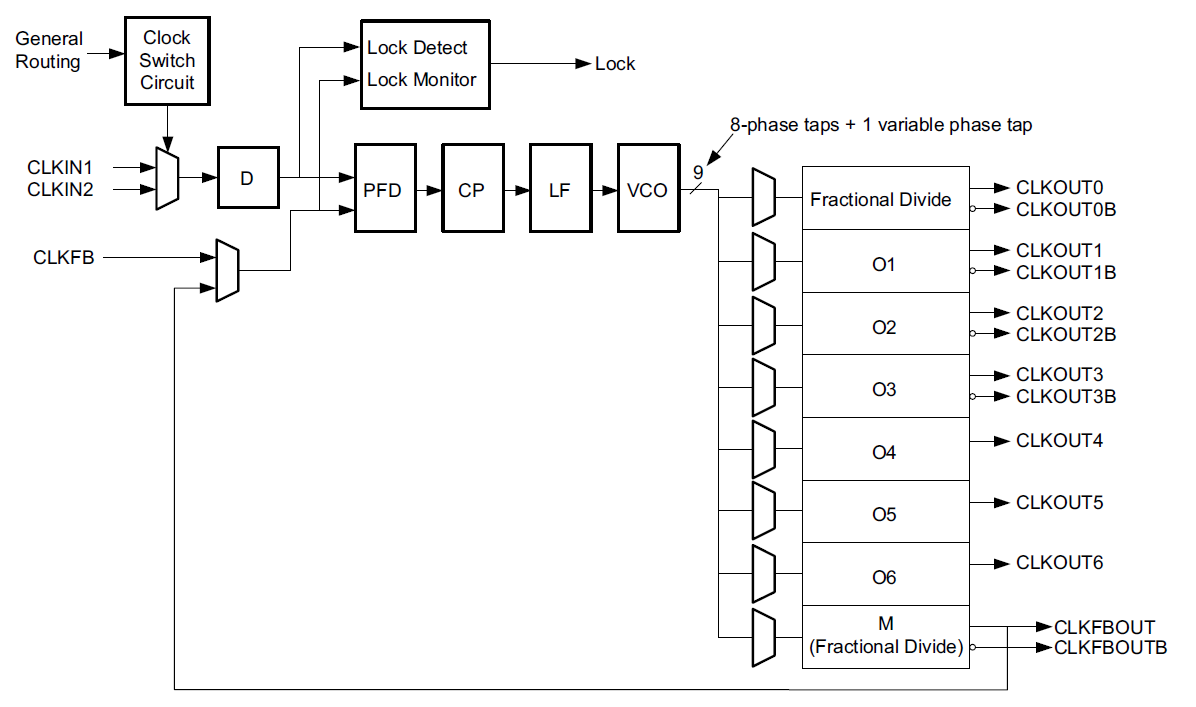
\includegraphics[width=\textwidth]{images/MMCM.png}
            \caption{MMCM Block Diagram}
            \label{MMCM}
        \end{center}
    \end{figure}

    \subsubsection{MMCM Primitives}
    The UltraScale device MMCM primitives, MMCME3\_BASE and MMCME3\_ADV. The UltraScale+ devices have the same primitives with an E4 instead of an E3. 

    \subsection{PLLs}
    There are two PLLs per CMT that provide clocking to the PHY logic and I/Os. In addition, they can be used as frequency synthesizers for a wide range of frequencies, serve as jitter  filters, and provide basic phase shift capabilities and duty cycle programming. The PLLs differ from the MMCM in number of outputs, cannot deskew clock nets, and do not have
    advanced phase shift capabilities, Multipliers and input dividers have a smaller value range and do not have many of the other advanced features of the MMCM.
    
    \subsubsection{PLL Primitives}
    The UltraScale device contain PLL primitives PLLE3\_BASE and PLLE3\_ADV.
    For UltraScale+ devices have the same primitives with an E4 instead of an E3. 

    \subsection{Dynamic Reconfiguration Port}
    \subsection{VHDL and Verilog Templates and the Clocking Wizard}
    \subsection{Clocking Guidelines}


    \clearpage

    \section{Question \& Answers}
	
    \begin{itemize}
        
        \question{What is the name of routing and clock resources?}
        \answer{Did not understand the question.}
        
        \question{Clock region and clock managment tile diagram?}
        \answer{The diagram represents half the FPGA. Better explanation with Xilinx video.}
        
        \question{BUFGCTRL Pins}
        \answer{ Selection of an input clock requires a "select" pair (S0 and CE0, or S1 and CE1) to be asserted High. If either S or clock enable (CE) is not asserted High, the desired input is not
        selected. In normal operation, both S and CE pairs (all four select lines) are not expected to be asserted High simultaneously. Typically, only one pin of a "select" pair is used as a select
        line, while the other pin is tied High.
        \begin{itemize}
            \item IGNORE: pins bypasses the BUFGCTRL from detecting the conditions for switching between
            two clock inputs.
            \item S:  is used to select a desired output and is also suggested for glitch-free switching.
            \item CE: is used to select a desired output. When using CE to switch clocks, the change in clock selection can be faster than when using S. A violation in the setup/hold time of the CE pins
            causes a glitch at the clock output. 
        \end{itemize}
        }
        
        \question{Why the clocks do not use I/O interconnects instead of clock interconnects?}
        \answer{Clock interconnects are designed to have low clock skew, low duty cycle distortion, and low power and improved jitter tolerence.}

    \end{itemize}
    

    \chapter{Zynq ultrascale+ MPsoc Memory Resources}
\end{document}



